Triangular centers and vertices sweep out, we've seen, beautiful curves elliptic or not. But one center took us aback. The locus of the {\em Mittenpunkt} $X_9$, where lines drawn from Excenters through side midpoints concur \cite{mw}, is {\em a point}, namely, the Billard center, Figure~\ref{fig:mitten} and \cite[video \#3]{dsr_main_videos_2019}.

\begin{theorem}
For an $N=3$ orbit family, the Mittenpunkt $X_9$ is stationary at the Billiard's center.
\end{theorem}

Stationarity of this point is a projective property of elliptic chords (irrespective of Billiards). A clever proof has been kindly contributed \cite{olga19_mitten} and is illustrated in Figure~\ref{fig:mitten-proof}. 


\begin{figure}[H]
     \centering
     \begin{subfigure}[t]{0.29\textwidth}
         \centering
         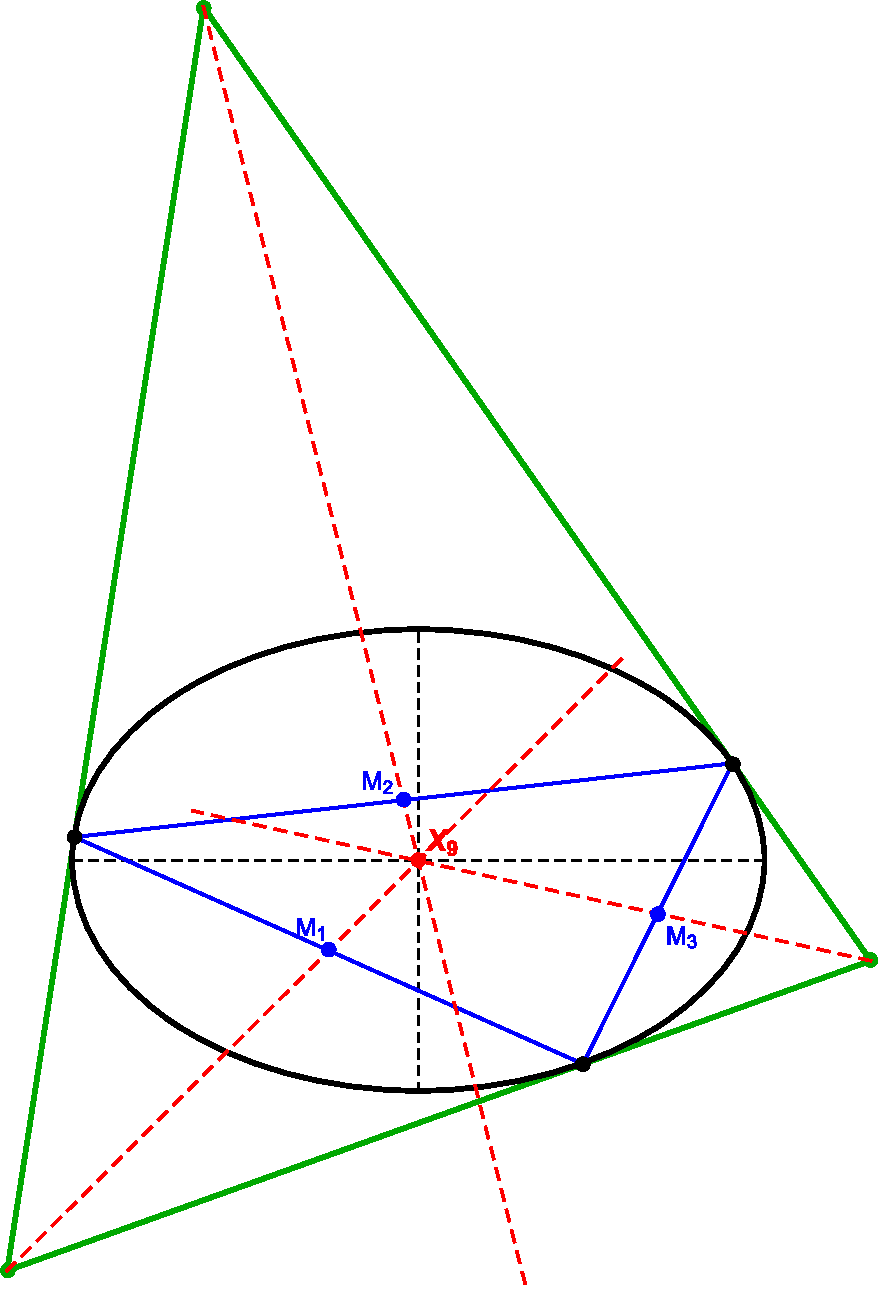
\includegraphics[height=1.75\linewidth]{pics/0051_mitten.pdf}
         \caption{An $N=3$ orbit (blue) and its Excentral Triangle (green), as well as the construction for $X_9$, the Mittenpunkt, located at the center of the Billiard (black).}
         \label{fig:mitten}
     \end{subfigure}
     \hfill
     \begin{subfigure}[t]{0.29\textwidth}
         \centering
         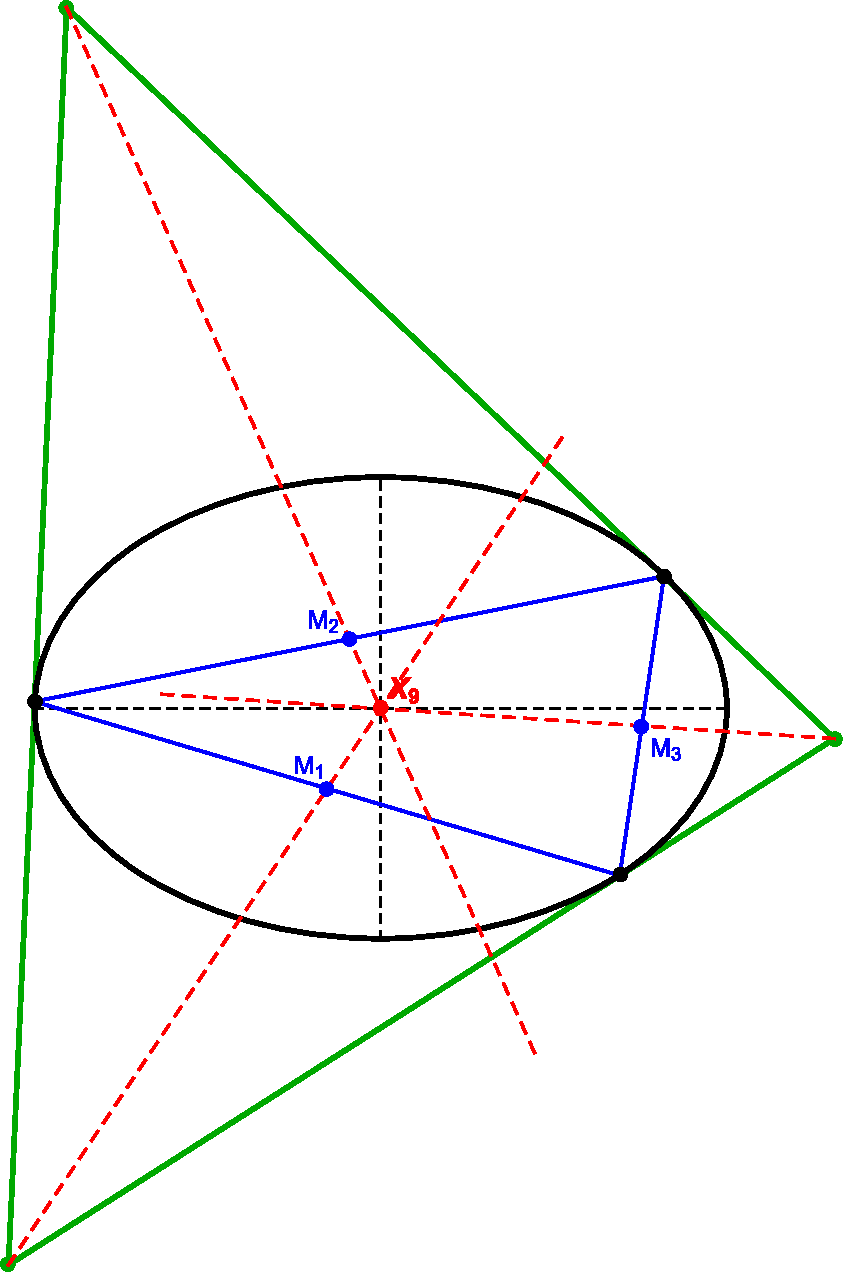
\includegraphics[height=1.75\linewidth]{pics/0052_mitten_rot.pdf}
         \caption{same construction for a slightly different orbit position, with $X_9$ unmoved.}
         \label{fig:mitten-rot}
     \end{subfigure}
     \hfill
     \begin{subfigure}[t]{0.29\textwidth}
         \centering
         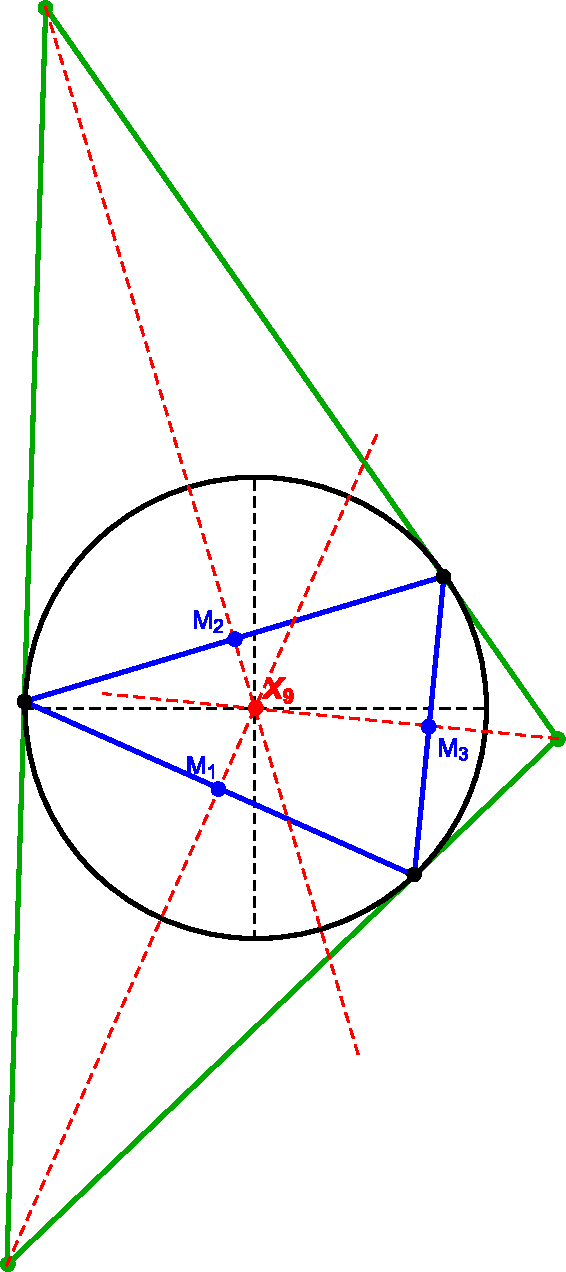
\includegraphics[height=1.75\linewidth]{pics/0053_mitten_rot_scaled.pdf}
         \caption{Affine transformation for which the Billiard becomes a circle, side midpoints become {\em chords} midpoints (distance ratios are preserved), and lines passing through transformed Excenters and chord midpoints concur at the circle center, uniquely identified under the transform with the Billiard center. 
         \label{fig:mitten-proof}}
     \end{subfigure}
     \caption{Left and Middle: Stationarity of the Mittenpunkt. Right: Proof via an Affine Transform.}
\end{figure}

\subsection{The Circumbilliard}

A triangle's {\em circumellipse} \cite{mw} passes through its three vertices. For $N=3$ orbits, we call this object a {\em Circumbilliard}. Since the orbit's Mittenpunkt $X_9$ is congruent with the Billiard's center, Figure~\ref{fig:circumbilliard}, we have:
%
\begin{observation}
Every triangle has a circumellipse to which it is a billiard orbit, whose center coincides with the triangle's Mittenpunkt.
\end{observation}
%
\begin{figure}[h]
    \centering
    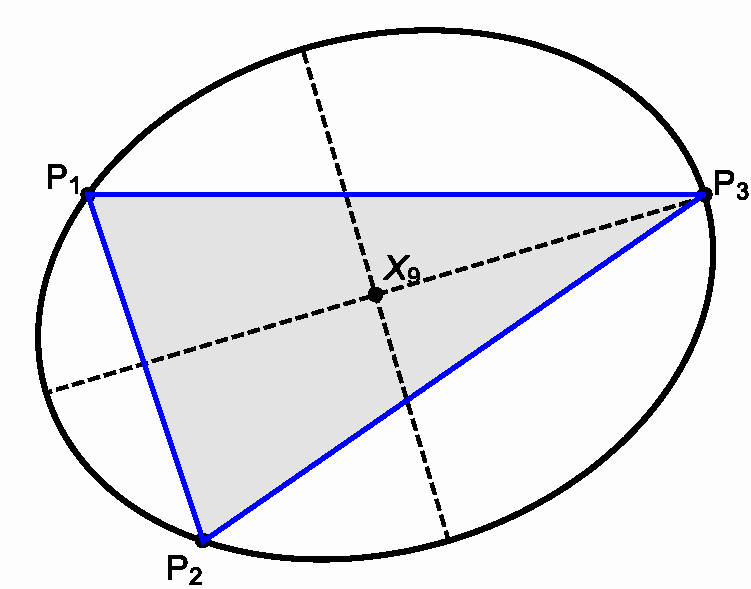
\includegraphics[width=.4\textwidth]{pics/0056_circumplot.pdf}
    \caption{A triangle's {\em Circumbilliard} is the circumellipse centered on $X_9$, the Mittenpunkt.}
    \label{fig:circumbilliard}
\end{figure}